% coding:utf-8

%----------------------------------------
%FOSADSVB, a LaTeX-Code for a summary of digital signal processing
%Copyright (C) 2015, Mario Felder & Michi Fallegger

%This program is free software; you can redistribute it and/or
%modify it under the terms of the GNU General Public License
%as published by the Free Software Foundation; either version 2
%of the License, or (at your option) any later version.

%This program is distributed in the hope that it will be useful,
%but WITHOUT ANY WARRANTY; without even the implied warranty of
%MERCHANTABILITY or FITNESS FOR A PARTICULAR PURPOSE.  See the
%GNU General Public License for more details.
%----------------------------------------

\chapter{Digtiales Filterdesign}
\begin{center}
	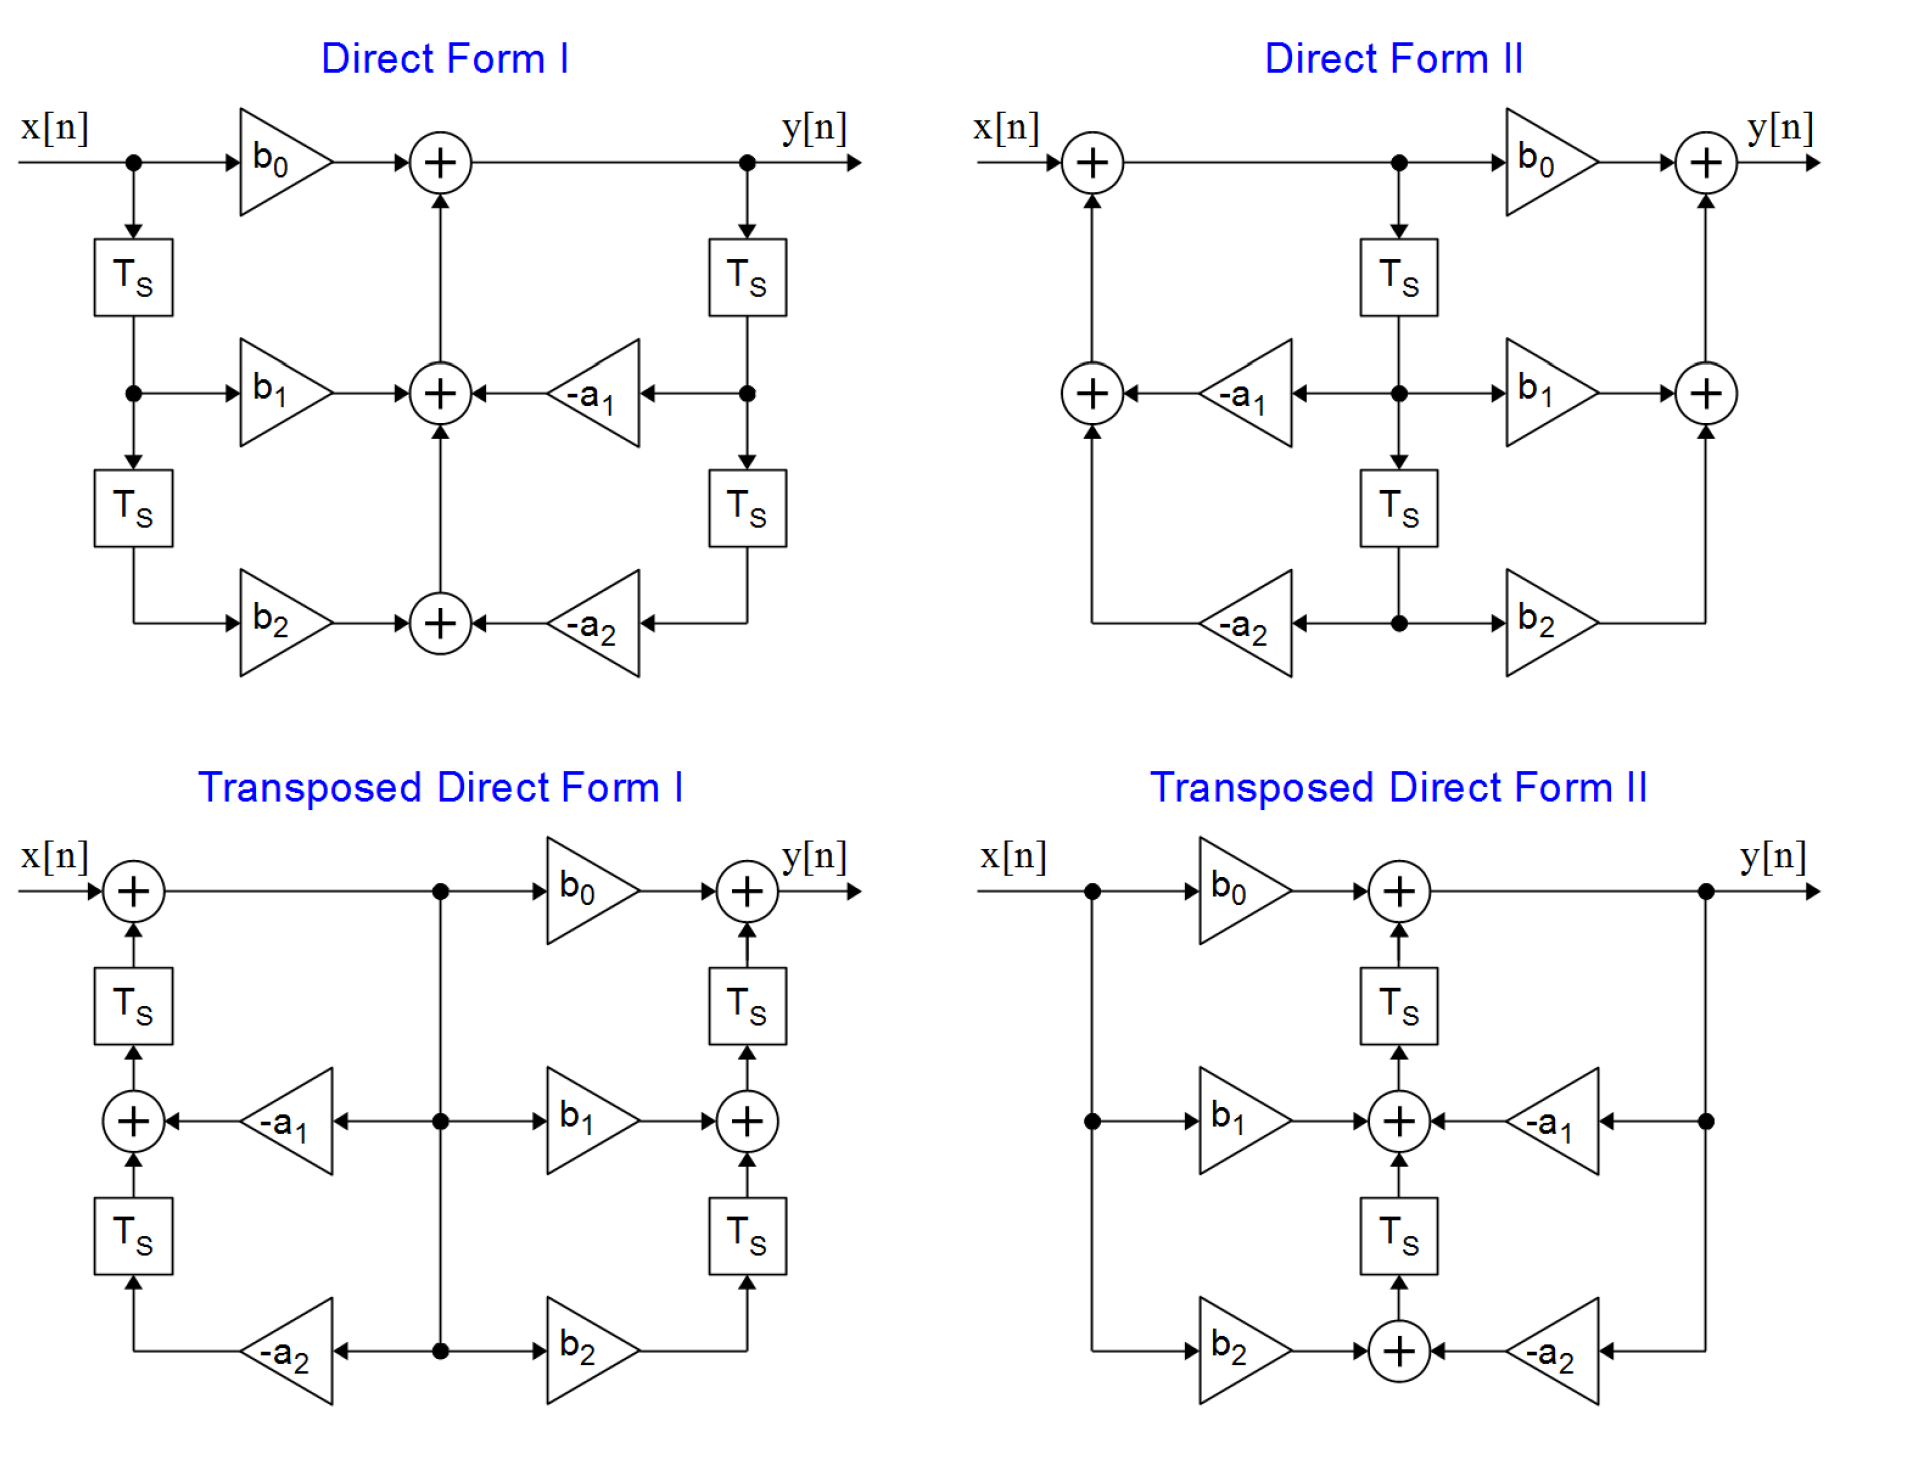
\includegraphics[scale=.8]{../fig/lti_scheme}
\end{center}
\section{FIR Filter}
FIR (finite impulse response) Filter der Ordnung $N$ hat folgende
Übertragungsfuntion:
\[ H(z) =b_0 + b_1z^{-1} + \ldots + b_Nz^{-N} \]
Die Impulsantwort ist $N+1$ Zeitschritte lang und entspricht den Koeffzienten
von $H(z)$:
\[ h[n] = \{ b_0,b_1,\ldots,b_N,0,0,\ldots \} \]\\
\\
\textrm{Stabilität:}\\
Da alle Pole bei $z=0$ liegen, sind FIR-Filter per Definition stabil.\\
\\
\textrm{Lineare Phase:}\\
Mit einem FIR-Filter is es einfach möglich, eine lineare Phasenübertragung
zu realisieren.\\
\\
\textrm{Implementation}\\
Die Realisierung von FIR-Filter in HW oder SW ist straightforward und unkritisch.

%===============================================================================
\subsection{Symetrische FIR-Filter}
Ein FIR-Filter ist symmetrisch wenn
\[ b_i = \pm b_{N-i} \qquad i = 0,1,\ldots,N \]
Wenn die gleichung mit "+" erfüllt ist, spricht man von einem symmetrischen 
FIR-Filter, wenn sie mit "-" erfüllt ist, spricht man von einem asymmetrischen.\\
\\
Alle symetrischen Filter haben eine lineare Phasenantwort im Pass-Band. Das
heisst, sie haben ein konstantes Gruppen-Delay:
\[ \tau_g = \frac{N}{2} \cdot T_S \]

\begin{center}
	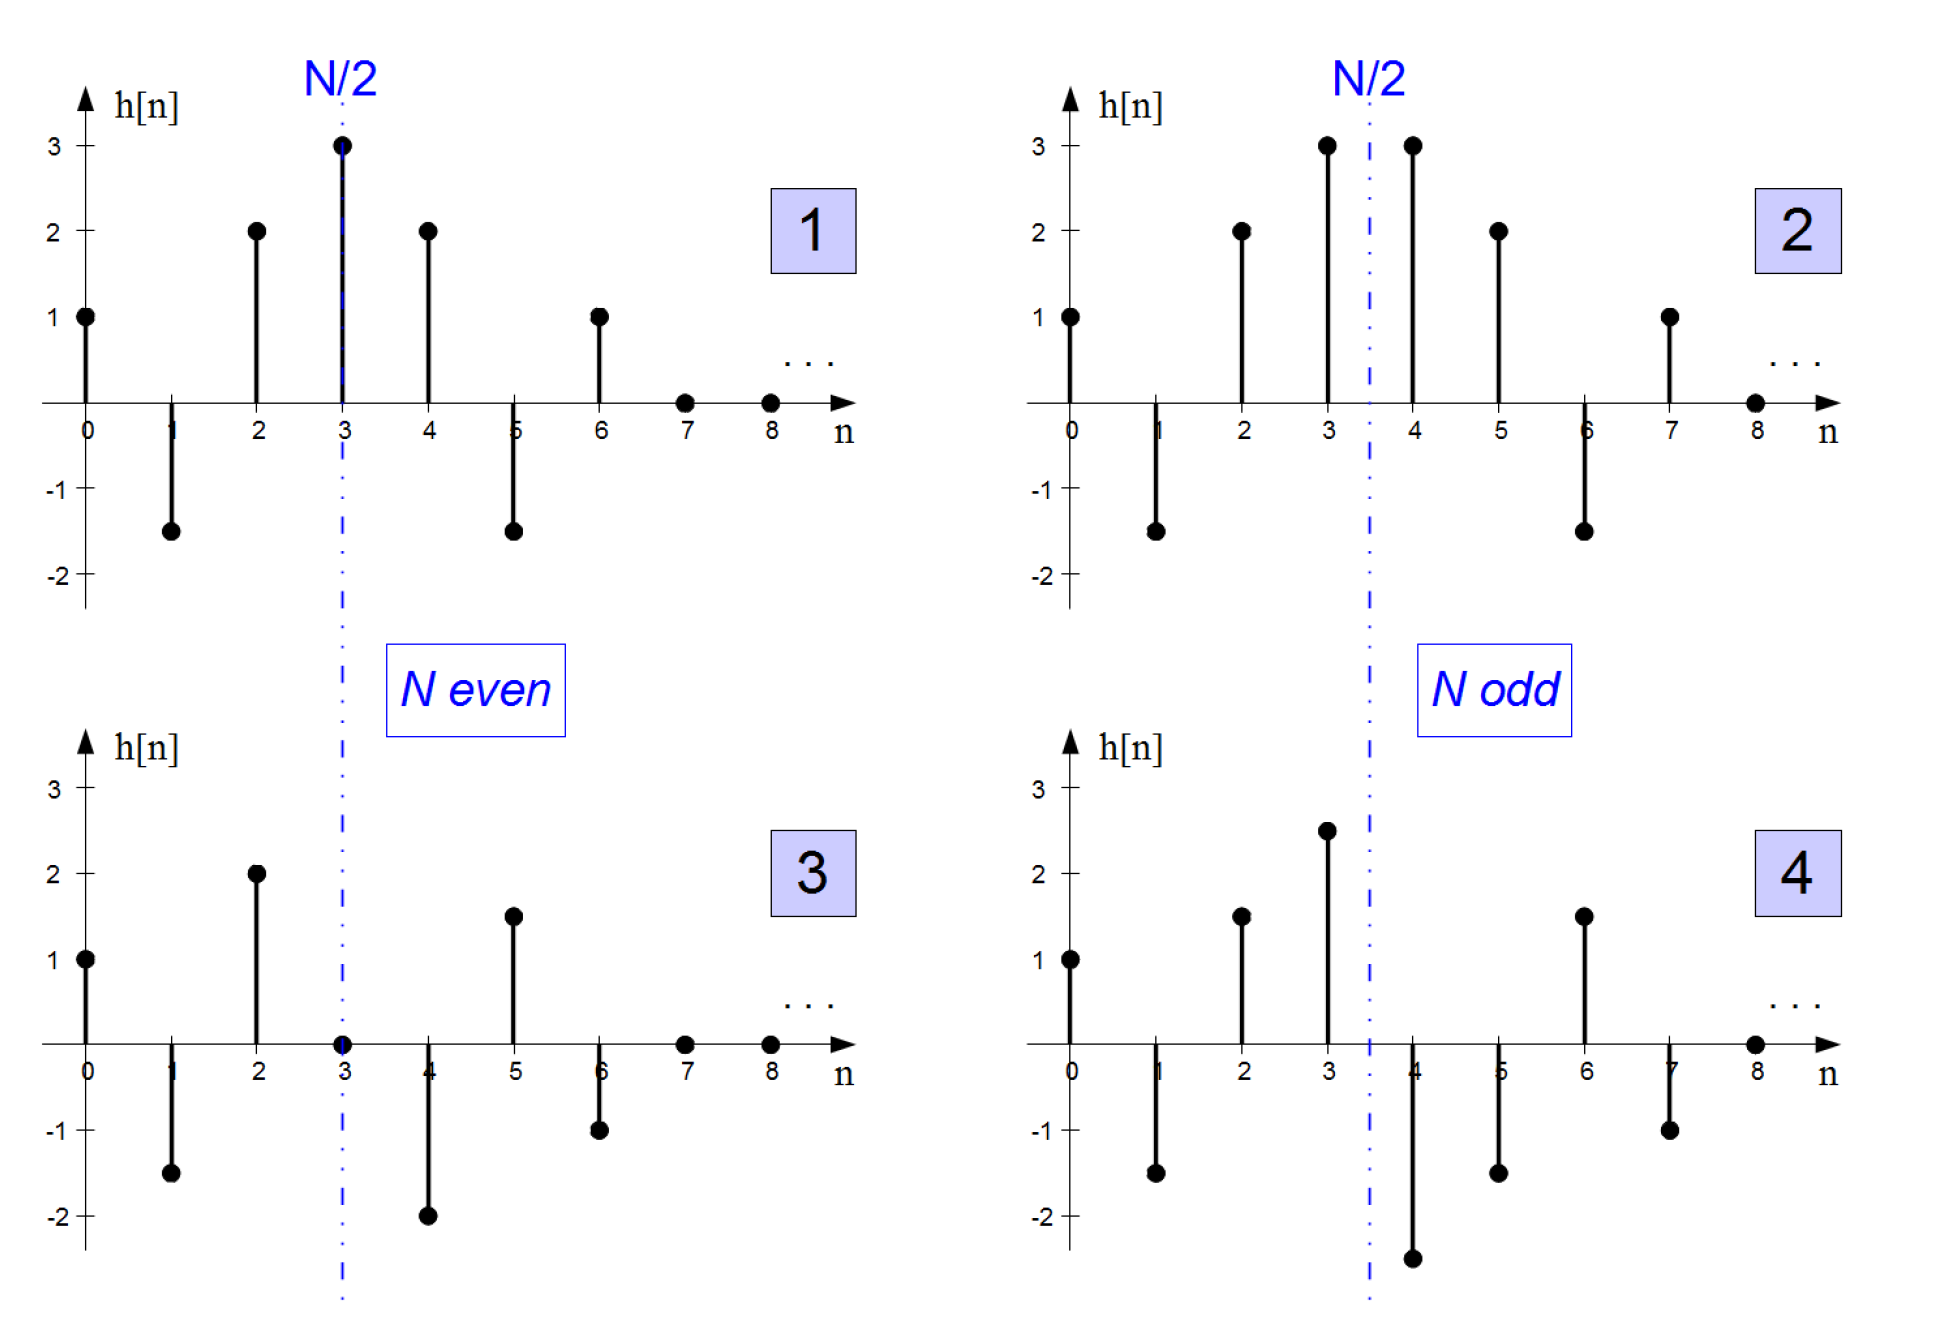
\includegraphics[scale=.7]{../fig/fir_filter}
	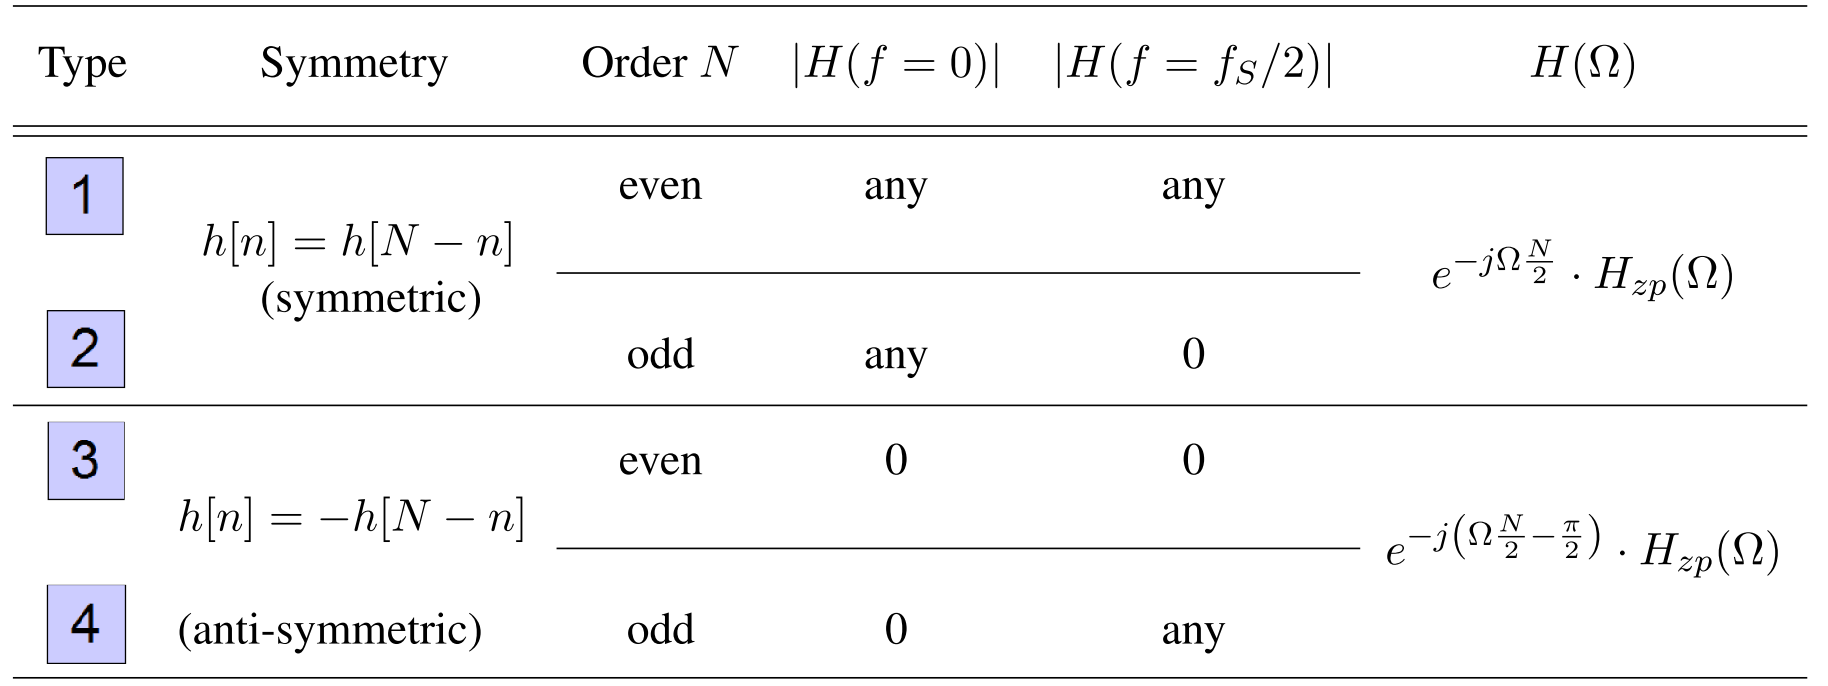
\includegraphics[scale=.7]{../fig/fir_table}
\end{center}

%===============================================================================
\section{IIR Filter}
\begin{center}
	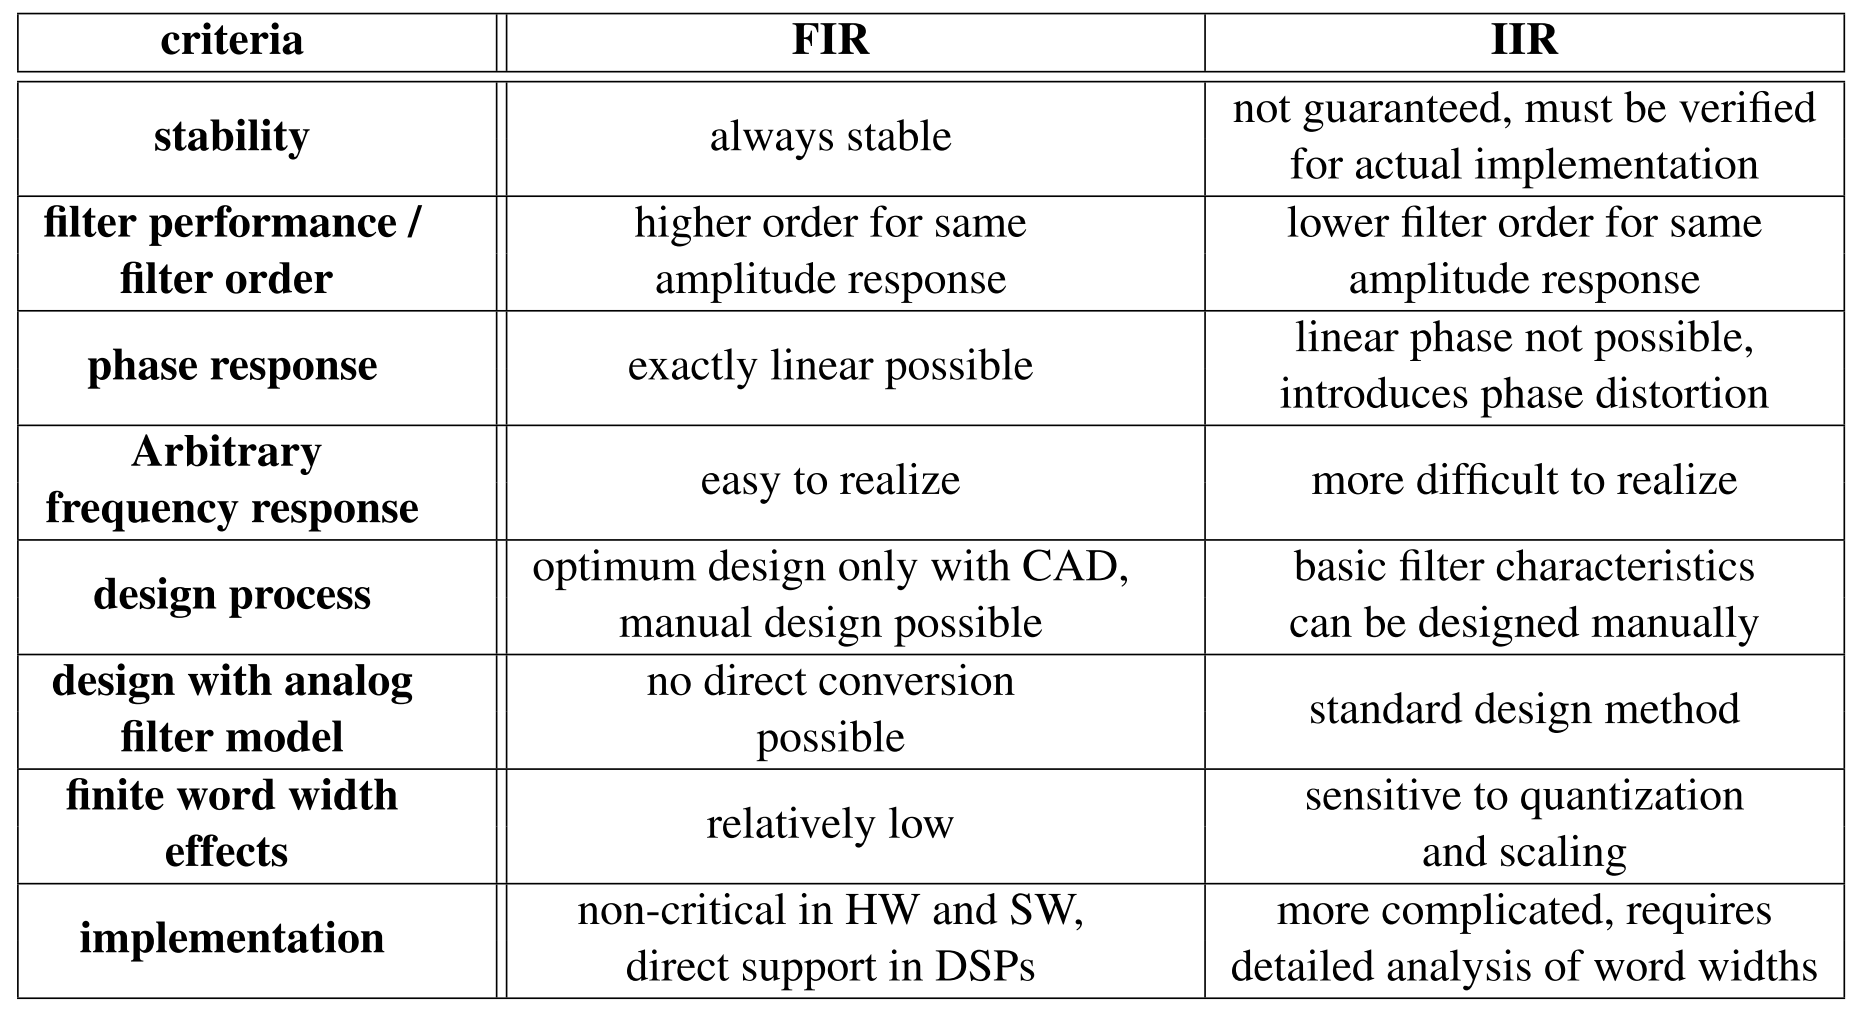
\includegraphics[scale=.7]{../fig/fir_vs_iir}
\end{center}
Umformung vom p-Plan zum z-Plan
\[ z = \e^{pT_S} \]
Der IIR Fitler kann als biquads implementiert werden. Dabei wird die
Übertragungsfunktion in mehrere aufgeteilt, welche jeweils einen Konjungert-
Komplexen Pol haben:
\[ H(z) = K \cdot \frac{(z-z_1)(z-z_1^*)}{(z-p_1)(z-p_1^*)}\cdot\ldots\cdot
	\frac{(z-z_L)(z-z_L^*)}{(z-p_L)(z-p_L^*)} \]
Bei einer Fix-Point Implementierung mit $W$ bits ($b_k$) und $F$ Nachkommastellen ist
der dezimale Wert:
\[ D_{ufix} = \sum_{k=0}^{W-1}b_k \cdot 2^{k-F} \]
Für Zahlen im Zweierkomplement:
\[ D_{fix} = -b_{W-1} \cdot 2^{W-F-1} + \sum_{k=0}^{W-2} b_k \cdot 2^{k-F} \]
